% Grundlagen für Arbeit (Related Work), Sehapparat, Raytracing, Volumenrendering, Eyetracking, GPU Architektur (Warps usw.) %

\chapter{Grundlagen}\label{chap::basics}
\label{chap:k2}
Dieses Kapitel beschäftigt sich mit den Grundlagen für diese Arbeit.
Der erste Abschnitt des Kapitels beschäftigt sich mit verwandten Arbeiten zum Thema Wahrnehmungsorientiertes Volumen-Rendering.
Der zweite Abschnitt handelt über die Grundlagen des menschlichen Sehapparates.
Hier werden die Fähigkeiten und Limitierungen der visuellen Wahrnehmung des Menschen diskutiert.
In Abschnitt drei, wird die Funktionsweise von Raytracing erläutert, welches ein grundlegender Algorithmus, der für diese Arbeit zugrunde liegender Implementierung ist.
Zusammenhängend mit Raytracing wird im Abschnitt vier, die Verwendung des Raytracers für das Volumenrendering erläutert.
Abschnitt fünf diskutiert die Auswahl des für diese Arbeit zugrunde liegenden Eyetrackers und dessen Verwendung für die Erfassung des fovealen und peripheren Bereichs.
Aus Performanzgründen kann es hilfreich sein für Berechnungen auf einer GPU, die Architektur der GPU zu betrachten und unter Umständen Algorithmen für eine bessere Effizienz anzupassen.
Diese Thematik wird in Abschnitt sechs behandelt.
\todo{Beschreibung der Grundlagen überarbeiten}

\section{Related Work}\label{sec::relwo}
Wahrnehmungsorientiertes Volumenrendering ist kein absolut neues Arbeitsgebiet und ist schon Teil einiger wissenschaftlicher Arbeiten gewesen \todo{Beispiele}.
Da diese Arbeit auf zwei trennbare Aspekte beruht, unterteile ich den Related Work Abschnitt in zwei Teile.
Der erste Abschnitt bezieht sich auf Arbeiten im Bereich des wahrnehmungsorientierten Renderings mit dem Ziel, die Performanz einer Anwendung zu steigern.
Die Ansätze hier beziehen sich meist darauf, dass die Qualität der Darstellung im peripheren Bereich der visuellen Wahrnehmung, gesenkt wird und so für die Berechnung eines Bildes weniger Rechenleistung aufgewendet werden muss.
\todo{Was genau ist mit Performanz gemeint?}
Der zweite Abschnitt bezieht sich auf Arbeiten zu wahrnehmungsorientiertem Volumenrendering, mit dem Ziel, die Qualität der Darstellung zu erhöhen.
Dabei werden vor allem Ansätze zur geschickten Anpassung von Parametern einer Transferfunktion vorgestellt, die dem Betrachter ein insgesamt besseres Verständnis der Volumendaten ermöglichen soll.
\subsection{Performanz- und Wahrnehmungsorientiertes Volumenrendering}
In einem Paper von Marc Levoy und Ross Whitaker \enquote{Gaze-Directed Volume Rendering} \cite{Levoy:1990:GVR:91385.91449} erforschten diese Methoden, wie Eyetracking-Daten in Rendering-Algorithmen eingesetzt werden könnnen.
Das Ziel ihrer Forschung war es, dem Nutzer einen Arbeitsplatz für Echtzeit-Volumen-Rendering, mit der Illusion eines hochauflösendes Bildes über den gesamten Bildschirm, zu präsentieren, welches durch Eyetracking unterstützten Verfahren einen geringeren Berechnungsaufwand als herkömmliche Volumen Renderer hat.
Dafür präsentierten sie eine Implementierung eines Ray-Tracers für Volumen Daten, in welcher mit Hilfe der Eyetracking-Daten der Blickfokus auf dem Bildschirm berechnet wurde und um diese Position herum, die Anzahl der Strahlen und die Samples pro Strahl, abhängig von der Distanz zum Blickfokus, angepasst wurden.
Die Implementierung basiert auf darauf, dass der Detaillgrad der visuellen Wahrnehmung des Menschlichen Auge nur in einem kleinen, zentralen Bereich, der Fovea, am höchsten ist und zu den Rändern des Blickfelds hin, der periphere Bereich, stark abnimmt.
Ausgehend davon, berechneten sie in dem von dem Nutzer fokussierten Bereich, das Bild mit der vollen Auflösung und einer hohen Abtastrate der Strahlen.
In dem restlichen Bereich reduzierten sie die Auflösung des Bildes und abhängig von dem Abstand eines Pixels zum Blickfokus, die Abtastrate eines Strahls.
In ihrer Implementierung verwendeten sie 2D und 3D mip maps, einen Eye Tracker und die Pixel-Planes 5 rendering engine, ein hoch paralleles Raster Display System.
Um die geringere Abtastung in der Peripherie gut nutzen zu können, wurde aus den 3D Volumendaten eine 3D mip map erstellt.
Die 3D mip map wird durch den Ray-Tracing Algorithmus abgetastet und durch trilineare Interpolation eine 2D mip map erstellt.
Die 2D mip map ist Grundlage für die Erstellung des endgültigen Bildes.
In ihren Ergebnissen konnten sie die Rendering Kosten für ein teilweise hochauflösendes Bild im Vergleich zu einem vollständig hochauflösenden Bildes, um bis den Faktor fünf, senken.

In einer Arbeit von Guenter et. Al. \enquote{Foveated 3D Graphics} \cite{foveated-3d-graphics}, wurde ähnlich zu dem Paper von Levoy und Whitaker, der Abfall der visuellen Auflösung des Auges außerhalb des visuellen Zentrums, der Fovea, ausgenutzt, um eine beschleunigte Berechnung des Bildes zu erhalten.
Im Gegensatz zu der davor genannten Arbeit, ist das darunterliegende System hier kein Ray-Tracer für Volumendaten, sondern eine Grafikpipeline für 3D Szenen.
Das Bild wird hier aus drei Teilbilder zusammengesetzt, welche jeweils mit unterschiedlichen Auflösungen berechnet wurden und wie Schichten übereinander gelegt werden.
Die drei Schichten sind: innere Schicht, mittlere Schicht und äußere Schicht.
Die innere Schicht hat ungefähr die Größe des fovealen Bereichs auf dem Bildschirm und wird in der maximalen Auflösung berechnet.
Ihr Mittelpunkt ist der Blickfokus des Betrachters.
Die mittlere Schicht ist ein bisschen größer als die innere Schicht und wird mit einer niedrigeren Auflösung berechnet. 
Sie wird ebenfalls auf den Blickfokus des Betrachters zentriert.
Die äußerste Schicht überdeckt den gesamten Bildbereich und wird in der niedrigsten Auflösung berechnet.
Um die Schichten zusammensetzen zu können, werden die mittlere und äußere Schicht jeweils zur nativen Auflösung des Bildschirms, die gleiche Auflösung wie die innere Schicht, interpoliert.
Scharfe Kanten zwischen den Schichten werden dadurch vermieden, dass diese sich leicht überlappen und spezielle Blend-Masken verwendet werden, um die verschiedenen Schichten glatt übereinander zu blenden.
In ihrer Arbeit nahmen sie sich auch das Problem an, dass das starke Unterabtasten, um bis zu dem Faktor sechs in jede Dimension, in der mittleren und äußeren Schicht zu störenden und sich bewegenden Artefakten führen kann.
Um dies entgegen zu wirken, verwendeten sie drei Antialiasing Techniken: Hardware Multi-Sample Antialiasing (MSAA), \enquote{Temporal Reprojection} und \enquote{whole frame jitter sampling}.
Um die Blickposition zu erfassen nutzten sie den Tobii Tx 300 Eye Tracker mit einer Worst-Case Latency von 10 ms.
Das Bild wurde auf einem Computer mit Intel Xeon CPU (E5640 mit 2.67 Ghz) und einer NVidia GeForce GTX 580 GPU berechnet.
Dargestellt wurde es auf einem 23" 1920x1080 LCD Monitor mit einer Bildwiederholungsrate von 120 Hz.
Mit ihrem System und Techniken erlangten sie eine Performanz-Verbesserung von einem Faktor zwischen fünf und sechs auf einem Monitor mit HD Auflösung.
Dabei erreichten sie eine Darstellungsqualität, die vergleichbar mit dem Rendern eines hochauflösenden Bildes über den gesamten Bildschirm ist.

\subsection{Wahrnehmungsorientiertes Volumenrendering zur Qualitätssteigerung}
R. Englund und T. Ropinski stellten in ihrem Paper \enquote{Quantitative and Qualitative Analysis of the Perception of Semi-Transparent Structure in Direct Volume Rendering} \cite{doi:10.1111/cgf.13320} verschiedene Techniken, zur Verbesserung der Wahrnehmung von komplexen volumetrischen Daten, vor.
In einer Studie mit über 300 Teilnehmern untersuchten sie, wie diese Techniken zur verbesserten Wahrnehmung von Volumen beitragen und verglichen die verschiedenen Ansätze miteinander.
Dabei mussten die Teilnehmer jeweils kleine Aufgaben absolvieren, so dass Rückschlüsse darauf geschlossen werden können, wie sehr eine gewisse Technik dem Teilnehmer bei der Erkennung von Form und Tiefe eines Objekts in einem Volumen beiträgt.
Um eine bessere direkte Erforschung der Volumen-Daten später ermöglichen zu können, wurden Techniken, die automatisch Rendering-Parameter angepasst haben hier ausgelassen.
Nur wenn der Nutzer selbst interaktiv sein kann, also die Parameter des Volumen-Renderings, wie die Transferfunktion und Kamera selbst anpassen kann, ermöglicht dies eine direkte Erforschung.
In ihrer Studie haben sie sechs Techniken ausgewertet. Darunter \enquote{Direct Volume Raytracing} (DVR) als grundlegende Technik und \enquote{Depth Darkening} wobei Tiefeneffekte ähnlich zu \enquote{Ambient Occlusion} dadurch hervorgerufen werden, dass tiefere Objekte dunkler gezeichnet werden. 
In ihrer Auswertung kamen sie unter Anderem dazu, dass Techniken, die natürliche Lichteffekte in den Volumendaten simulieren, deutliche Vorteile gegenüber die anderen getesteten Ansätze gezeigt haben.

Anders als zu den untersuchten Techniken von Englund und Ropinski \cite{doi:10.1111/cgf.13320} präsentieren Aidong Lu et. Al. in ihrem Paper \enquote{Volume Composition Using Eye Tracking Data} \cite{Lu:2006:VCU:2384796.2384814} eine Methode für automatisierte Parameterauswahl bei der Betrachtung von Volumen Daten mit Hilfe eines Eye Tracking Gerätes.
Das Ziel, welches sie mit dieser Methode verfolgen ist es, die mühsame Nutzerinteraktionen bei der Auswahl der Parameter zu vereinfachen und damit die Nutzbarkeit des Darstellungssystems zu verbessern.
Volumen Daten können sehr komplex sein und daher ist es oft schwierig herauszufinden, was der Nutzer in dem Volumen betrachten möchte und was dahingehend hervorgehoben werden soll.
Trotzdem ermöglichen Eigenschaften des Volumen Renderings, wie konstante Größen, Formen und Positionen der Objekte eine automatische Anpassung der Parameter.
Um die Bereiche, die für den Nutzer von Interesse sind, zu bestimmen, wird ein Eyetracker zur Hilfe genommen.
Dieser misst die Augenbewegungen und die Blickposition auf dem Bildschirm.
Es wird zwischen zwei Hauptsächlichen Augenbewegungen unterschieden: Sakkade und Fixation.
Eine Sakkade ist eine schnelle Augenbewegung von einem Punkt zu einem anderem.
Bei einer Fixation ruht das Auge auf einem Punkt.
Die Punkte, die fixiert werden, sind meist für den Nutzer von Interesse.
Da die Blickposition durch den Eye Tracker nur auf einer 2D-Ebene bestimmt werden kann, wird durch ein konstantes Rotieren des Volumen Objekts und der parallelen Aufzeichnung der Augenbewegung versucht, die 3D Position des fixierten Objektes zu rekonstruieren.
Aus den Eyetracking und Volumendaten bestimmen sie mit Hilfe mehrerer Clustering-Methoden gewichte für die einzelnen Voxel des Volumens und berechnen so die Wichtigkeit der Objekte innerhalb des Volumens für den Nutzer.
Entsprechend dieser Ergebnisse wurden die Render Parameter angepasst, um die für den Nutzer am interessantesten Objekte hervorzuheben und anzuzeigen.
Aidong Lu et. Al. kamen zu dem Schluss, dass die präsentierte Methode den Aufwand für den Nutzer, die Render Parameter anzupassen, signifikant reduzieren kann.
Trotzdem kann ein solcher regelbasierter Ansatz nicht mit einer manuellen Einstellung der Render-Parameter mithalten.
\todo{Related Work nochmal anschauen. Zum Bsp. ob aus der richtigen Perspektive geschrieben wurde.}

\section{Sehapparat}\label{sec::eye}
Das Auge ist der visuelle Sensor des Menschen und ermöglicht ihm das Sehen.
Wahrnehmungsorientiertes Rendering nutzt gezielt Eigenschaften der visuellen Wahrnehmung des Menschen aus.
Dafür ist es notwendig, ein gutes Verständnis des menschlichen visuellen Wahrnehmungsapparates zu besitzen.
In diesem Abschnitt stelle ich einige Eigenschaften des visuellen Wahrnehmungsapparates vor, wie sie in \cite{doi:10.1111/cgf.13150} vorgeführt werden.
\begin{figure}
	\centering
	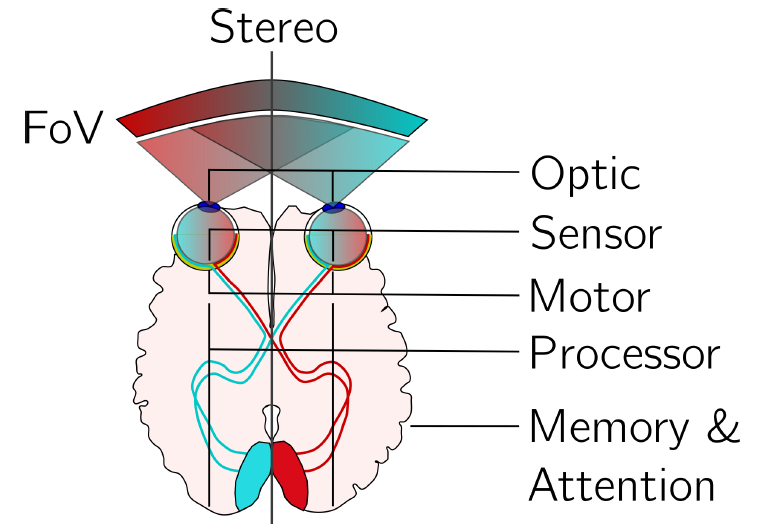
\includegraphics[width=0.5\textwidth]{../../Grafiken/HVS-model_from-star-report.png}
	\caption{Modell des visuellen Wahrnehmungsapparates des Menschen aus \cite{doi:10.1111/cfg.13150}}
	\label{fig::eye01}
\end{figure}
Abbildung \ref{fig::eye01} ist ein Modell des visuellen Wahrnehmungsapparates des Menschen.
Das Modell unterteilt den Sehapparat des Menschen in Optik, Sensorik, Motorik, Verarbeitung, Speicherung und Aufmerksamkeit.
Licht trifft auf die Augen und wird durch die Optik auf die Retina, die Sensorik, weitergeleitet.
Hier wird der visuelle Input abgetastet und gefiltert.
Dabei entstehen zwei Datenströme welche die Verarbeitung stereoskopischer Bilder über einen großen Blickwinkel mit unterschiedlichen räumlich unterschiedlicher Auflösungen ermöglichen.
Die Retina (oder auch Netzhaut) ist mit dem visuellen Kortex verbunden.
Die Signale werden über die visuellen Nerven komprimiert und zum visuellen Kortex transportiert.
Dort werden sie von verschiedenen Bereichen im Gehirn verarbeitet.
Speicherung und Aufmerksamkeit spielen dabei eine wesentliche Rolle.

Das visuelle Wahrnehmungssystem des Menschen hat wesentliche Limitierungen, die bei der Darstellung von Bildern gezielt genutzt werden können.
Die Sehschärfe des ungleich auf der Retina verteilt und nur in in einem kleinen, zentralen Bereich ist die Sehschärfe maximal.
Dieser Bereich wird Fovea oder auch Gelber Fleck genannt.
Je weiter man sich von der Fovea nach außen hin entfernt, desto mehr nimmt die Sehschärfe ab.
Der Bereich um die Fovea ist der periphere Bereich des Auges.
% Eine Verringerung der Bildqualität ist daher im äußeren Bereich möglicherweise nicht wahrnehmbar.
% Diese Eigenschaft motiviert den Versuch, die Bildqualität im peripheren Bereich zu reduzieren, um ohne merkliche Verluste in der visuellen Wahrnehmung des Betrachters den Rechenaufwand des Renderings zu reduzieren.
Das Sichtfeld des visuellen Wahrnehmungsapparates des Menschen ist bei gerade gerichteten Blick horizontal bis circa 190\textdegree{} und mit Augenrotation bis zu 290\textdegree{}.
Visuelle Reize werden über das gesamte Sichtfeld wahrgenommen.
Abhängig von dem zuständigen Bereich auf der Retina gibt es starke Unterschiede, wie die visuellen Reize über das Sichtfeld verteilt, verarbeitet werden.
Durch das Verkleinern (Miosis) und Vergrößern (Mydriasis) der Pupille wird die Menge des einfallenden Lichts in das Auge gesteuert.
Die Pupille nimmt dabei Größen zwischen 2mm und 8mm Durchmesser an.

Die Netzhaut (Retina) ist die photosensitive Schicht des Auges und besteht aus zwei Typen von Photorezeptoren, aus Zapfen und Stäbchen.
Es sind circa $6*10^6$ Zapfen und ungefähr 20 mal so viele Stäbchen auf der Retina verteilt.
Stäbchen sind für die Helligkeitswahrnehmung verantwortlich.
Zapfen sind für die Farbwahrnehmung verantwortlich.
Man unterscheidet zwischen drei Zapfentypen: L-Zapfen für lange Wellenlängen, M-Zapfen für mittlere Wellenlängen und S-Zapfen für kurze Wellenlängen.

Die Fovea ist der Bereich um circa 5,2\textdegree{} um das Zentrum der Retina und besteht fast ausschließlich aus Zapfen.
Die Anzahl der Zapfen nimmt aber nach außen hin stark ab.
Der Bereich von circa 5,2\textdegree{} bis 9\textdegree{} wird als Parafovea bezeichnet.
Der Bereich zwischen circa 9\textdegree{} bis 17\textdegree{} heißt Perifovea.
Fovea, Parafovea und Perifovea sind für die zentrale Sicht verantwortlich.
Alles außerhalb ist die periphere Sicht.
\begin{figure}
	\centering
	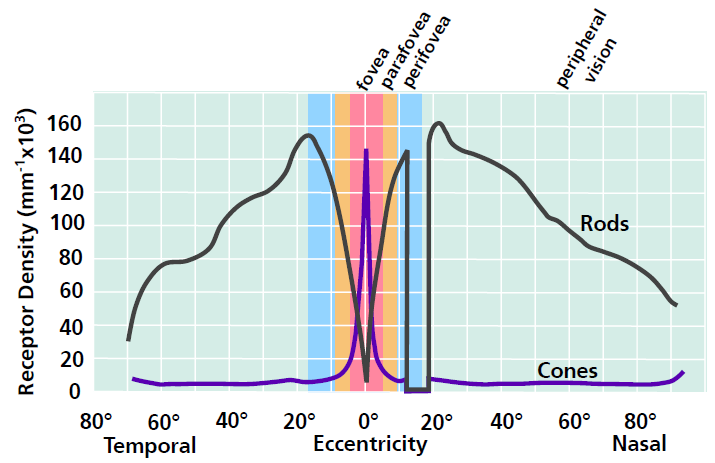
\includegraphics[width=0.5\textwidth]{../../Grafiken/Retinal-photoreceptor-distr_from-star-report.PNG}
	\caption{Verteilung der Photorezeptoren auf der Retina \cite{doi:10.1111/cfg.13150}}
	\label{fig::eye02}
\end{figure}
Abbildung \ref{fig::eye02} zeigt die Dichteverteilung der Photorezeptoren auf der Retina.
Die höchste Dichte der Stäbchen liegt bei circa 15\textdegree{} bis 20\textdegree{} um die Fovea herum.
Ihre Anzahl verringert sich nach außen hin circa linear.
Zapfen und Stäbchen sind sehr unterschiedlich auf der Reitna Verteilt.
Beide folgen aber einem Poisson-Disc Verteilungsmuster.
Die Dichte der Zapfen ist direkt mit der Sehschärfe verknüpft.
Daher fällt die Sehschärfe auch nach außen hin stark ab.
Bei 6\textdegree{} weg vom Zentrum beträgt die Sehschärfe schon nur noch ein Viertel der maximalen Sehschärfe.
Die Sehschärfe hängt aber auch von der Kontraststärke der visuellen Reize ab.
Dabei ist die Kontrastsensitivität von der Anzahl der auf den Reiz reagierenden neuronalen Zellen abhängig, welche ebenfalls nach außen hin stark abnimmt.
Die Farbsensitivität ist von der Verteilung von Stäbchen und Zapfen abhängig.
Die Zapfen zur Erkennung von grünem und rotem Licht sind vermehrt in der Fovea und eher weniger im peripheren Bereich verteilt.
Von allen Zapfen sind lediglich neun Prozent zur Erkennung von blauem Licht.
Diese sind vermehrt im peripheren Bereich verteilt als im Zentrum.
Rezeptoren im Auge passen sich deutlich schneller an die Helligkeit als an die Dunkelheit an.

Das Auge ist dauerhaft in Bewegung.
Sechs externe Muskeln ermöglichen es verschiedene Objekte von Interesse (OvI) in die Fovea zu bringen und zu fokussieren.
Die wichtigsten Arten von Augenbewegungen sind: Sakkaden, Vestibular-Okularer Reflex, weiche Augenverfolgung (Smooth pursuit eye motion (SPEM)) und (coupled vergence-accommodation motion).
\todo{Englische Begriffe richtig übersetzen.}
Der Vestibular-Okulare Reflex passiert relativ schnell mit einer Latenz von 7ms - 15ms und ermöglicht auch bei schnellen Kopfbewegungen OvI zu fixieren.
Der SPEM ermöglicht die weiche Verfolgung eines sich bewegendes Objektes.
Bei der Wahrnehmung der Umgebung ist die Sakkade und Fixation die wichtigsten Eigenschaften des Auges.
Eine Sakkade bezeichnet das schnelle springen von einem Ovi zu einem anderen.
Dabei erreicht das Auge Geschwindigkeiten von bis zu 900\textdegree/s.
Die Sehsensivität ist während einer solchen Sakkade stark geschwächt (saccade suppression).
Eine Fixation dauert zwischen 100ms - 1.5s.
Sie tritt meist dann auf, wenn ein OvI genauer betrachtet wird und die Augen darauf ruhen.
In natürlichen Szenen treten zwei bis drei Sakkaden pro Sekunde auf, mit jeweils durchschnittlich 250ms Fixationszeit.
Der räumliche Abstand zwischen den Fixierungen beträgt dabei circa 7\textdegree{}.
Ein Abstand von mehr als 30\textdegree{} wird als unangenehm empfunden und hat meist eine Kopfbewegung zur Folge.
Auch während einer Fixierung macht das Auge wichtige kleine Bewegungen, sogenannte Tremor Bewegungen.
Werden diese bewusst unterdrückt, resultiert dies in einem schwindenden Bild.
Kleinere Augenbewegungen von bis zu 2.5\textdegree{}/s haben kaum einen Effekt auf die Sehschärfe.

Das die Fovea einen sehr wichtigen Teil der visuellen Informationen liefert spiegelt sich auch darin wieder, dass über 30 Prozent des primären Sehverarbeitungsbereichs des Gehirns für die zentralen 5\textdegree{} des Sehfeldes, der Fovea, zuständig sind.
Der periphere Bereich ist hier benachteiligt, liefert aber trotzdem einen großen und wichtigen Teil der Informationen.
Besonders für das (frühe) Erkennen von Kontrasten, Objekten und Tieren.
%Farbveränderungen im peripheren Bereich haben einen größeren Einfluss als eine Veränderung der Ausrichtung \todo{Dieser Satz: richtig übersetzt / verstanden? Was heißt "Orientation" hier?}.
Aus dem peripheren Bereich werden auch wichtige kontextuelle Informationen geliefert.
Dies ermöglicht unter Anderem die Vorverarbeitung von Informationen.

Die Aufmerksamkeit spielt eine wichtige Rolle in der Verarbeitung von visuellen Stimuli. % Selective attention, focused attention, divided attention.
Visuelles tunneling bezeichnet das längere Fokussieren auf einen bestimmten Punkt, wodurch ein Großteil der peripheren Informationen nicht mehr oder stark reduziert wahrgenommen werden.
Die visuelle Auflösung reduziert sich circa linear für die ersten 20-30\textdegree{}.
Jedes lineare Modell für das visuelle Wahrnehmungssystem des Menschen ist aber immer nur eine Annäherung.
Farben haben einen großen Einfluss auf die Wahrnehmung von Kontraste.
Die Bewegungserkennung ist sowohl in der Fovea als auch im peripheren Bereich ähnlich oder genauso gut.
\todo{Grundlagen zum menschlichen Sehapparat überarbeiten: Teilweise sind Sätze zusammenhangslos aneinandergereiht. Hier eine bessere Verknüpfung finden.}

\section{Volumenrendering und Transferfunktion}\label{sec::voltff}
Es ist nicht trivial, 3D Volumendaten auf einem 2D Bildschirm informativ zu präsentieren.
In einem Volumen gibt es möglicherweise mehrere für den Betrachter interessante Objekte, welche sich durchaus gegenseitig überdecken können.
Daher stellt sich die Frage, wie die Volumendaten auf dem Bildschirm projiziert werden und dabei für den Betrachter auch Informationen an verschiedenen Positionen innerhalb des Volumen sichtbar gemacht werden können.
Raycasting ermöglicht in Verbindung mit einer Transferfunktion, ein Volumen auf eine 2D Ebene zu projizieren und dabei einzelne Bereiche des Volumens farbig hervorzuheben oder transparent erscheinen zu lassen.

\subsection{Raycasting}\label{sec::rc}
Raycasting ist ein Verfahren um Volumendaten abzutasten und auf eine 2D Rastergrafik zu projizieren.
Wie beim Raytracing werden beim Raycasting auch Sichtstrahlen verfolgt.
Die Sichtstrahlen werden dabei ausgehend von einer virtuellen Kamera im Raum verfolgt.
\begin{figure}[]
	\centering
	\begin{minipage}[b]{0.49\textwidth}
		\centering
		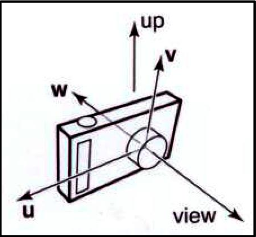
\includegraphics[width=0.5\textwidth]{../../Grafiken/Virtuelle-Kamera.PNG}
		\caption{Illustration einer virtuellen Kamera im Raum \cite{Dr.MichaelKrone2016/2017}}
		\label{fig::rc01}
	\end{minipage}
	\hfill
	\begin{minipage}[b]{0.49\textwidth}
		\centering
		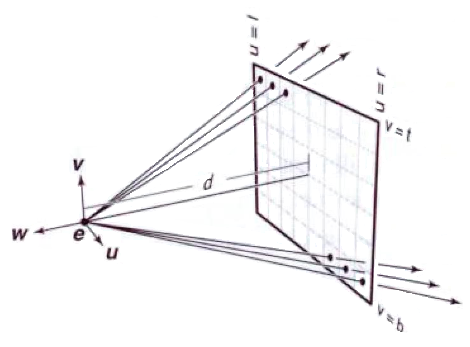
\includegraphics[width=1\textwidth]{../../Grafiken/Virtuelle-Kamera-und-Bildebene.PNG}
		\caption{Illustration der virtuellen Kamera und der Bildebene \cite{Dr.MichaelKrone2016/2017}}
		\label{fig::rc02}
	\end{minipage}
\end{figure}
Die virtuelle Kamera, siehe Abbildung \ref{fig::rc01}, ist im Raum an Position \texttt{e} positioniert, dies ist auch das Projektionszentrum, falls es keine orthogonale Projektion ist.
Die Position \texttt{e} entspricht relativ der Position des Betrachters vor dem Bildschirm.
Mit \texttt{u}, \texttt{v} und \texttt{w} wird die Ausrichtung der Kamera im Raum eindeutig bestimmt.
In einer Entfernung \texttt{d} von \texttt{e} aus in Richtung \texttt{-w} ist die Bildebene \ref{fig::rc02} Positioniert.
Die Größe der Bildebene wird durch \texttt{l}, \texttt{r}, \texttt{b} und \texttt{t} bestimmt.
Abhängig von der Größe des Bildschirms oder der Größe der gewünschten Rastergrafik, wird die Bildebene virtuell in die gewünschte Anzahl an Pixel in die Breite und Höhe unterteilt.
Jeder dieser Teile entspricht nun einem Pixel der Rastergrafik.
Nun kann für jeden Pixel ein Strahl, ausgehend von \texttt{e}, in Richtung des entsprechenden Punktes auf der Bildebene, ausgesendet und verfolgt werden.
\begin{figure}
	\centering
	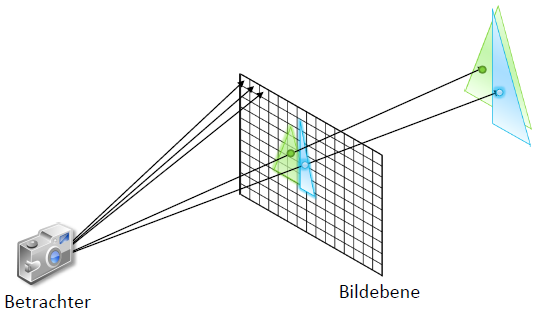
\includegraphics[width=0.5\textwidth]{../../Grafiken/Raytracing.png}
	\caption{Illustration der Projektion von Objekten auf die Bildebene mit Hilfe von Raytracing. \cite{Dr.MichaelKrone2016/2017}}
	\label{fig::rc03}
\end{figure}
Trifft ein Strahl Objekte in der Szene, wird dadurch ein Farbwert ermittelt, den der entsprechende Pixel annehmen kann und und die Szene dadurch auf den Bildschirm projiziert wird.
Siehe auch Abbildung \ref{fig::rc03}.
\todo{Grundlagen zu Raycasting hier. Vektoren als richtige Vektorensymbole darstellen (mit Pfeil oben drauf).}

\subsection{Volumenrendering}
Ein Volumen kann mit Hilfe von Raycasting abgetastet und auf den Bildschirm projiziert werden.
Hier wird wie beschrieben, für jeden Pixel ein Strahl in die Szene gesendet.
Anstelle von verschiedenen Objekten gibt es nun ein Volumen welches aus vielen kleinen Voxeln besteht.
Das Volumen ist ein dreidimensionales Bild, wobei statt 2D Pixel es aus 3D Voxel besteht.
Ein Voxel ist eine Box in dem Volumen, mit einer Position, einer Ausdehnung in drei Dimensionen und einer Dichte.
Wird ein Strahl in das Volumen gesendet, so wird dieser in Intervallen abgetastet.
Für jeden Abtastpunkt kann mit Hilfe einer Transferfunktion ein Farbwert ermittelt werden, welche zusammen einen Farbwert für den Pixel ergeben.
\todo{Anwendung von Raycasting zum Volumenrendering. Illustration von Rayasting und Volumenrendering mit mehreren Raysamples einfügen.}

\subsection{Transferfunktion}
Die Transferfunktion ist ein mächtiges Werkzeug für die Visualisierung von Volumendaten.
Mit Hilfe einer Transferfunktion können bestimmte Bereiche des Volumen verschieden stark ausgeblendet, oder auch farbig dargestellt werden.
Die Transferfunktion bestimmt für einen Voxel, abhängig von seiner Dichte, einen Farb- und Opazitätswert.
Dadurch können zum Beispiel Strukturen innerhalb des Volumens mit einer hohen Dichte farbig und kräftig hervorgehoben werden.
Strukturen mit einer geringeren Dichte können transparent und weniger farblich dargestellt werden.
\todo{Funktion der Transferfrunktion im Volumenrendering erläutern. Unter Umständen ein Beispiel Bild mit einer Anwendung der Transferfunktion verwenden.}

\section{Eyetracking}\label{sec::eyetr}
% \todo{Was ist Eyetracking?}
Für einige wahrnehmungsorientierte Methoden ist es notwendig, den aktuellen Blickpunkt des Betrachters auf dem Bildschirm zu wissen und daher die Augenaktivitäten zu messen.
In diesem Zusammenhang fällt meistens der Begriff \texttt{Eyetracking}.
Aber was ist Eyetracking?
Eyetracking ist das Messen von Augenaktivitäten eines Betrachters.
In der Regel betrachtet der Betrachter dabei einen Bildschirm während seine Augenaktivität gemessen werden, wodurch Informationen über den Blickverlauf und die Fixationsdauer bestimmter Punkte auf diesem Bildschirm errechnet werden können.
Diese Informationen ermöglichen es, Rückschlüsse über das betrachtete Bild zu ziehen, wie zum Beispiel, welche Objekte eines Bildes besonders interessant für den Betrachter sind.
Eyetracking ermöglicht aber nicht nur das Messen von Daten um diese im Nachhinein auszuwerten, sondern auch das Nutzen solche Daten für interaktive Anwendungen in Echtzeit.
Da in dieser Arbeit ein externer Tobii Eye Tracker verwendet wurde, beziehen sich folgende Informationen hauptsächlich aber nicht ausschließlich auf Tobii Eyetracker.
Die Firma Tobii AB schreibt auf ihrer Webseite zum Thema: Was ist Eyetracking?, dass Eye Tracking eine Technologie ist, die es ermöglicht, ein Gerät durch die natürliche Bewegung der Augen zu steuern \cite{tobii}.
\begin{figure}
	\centering
	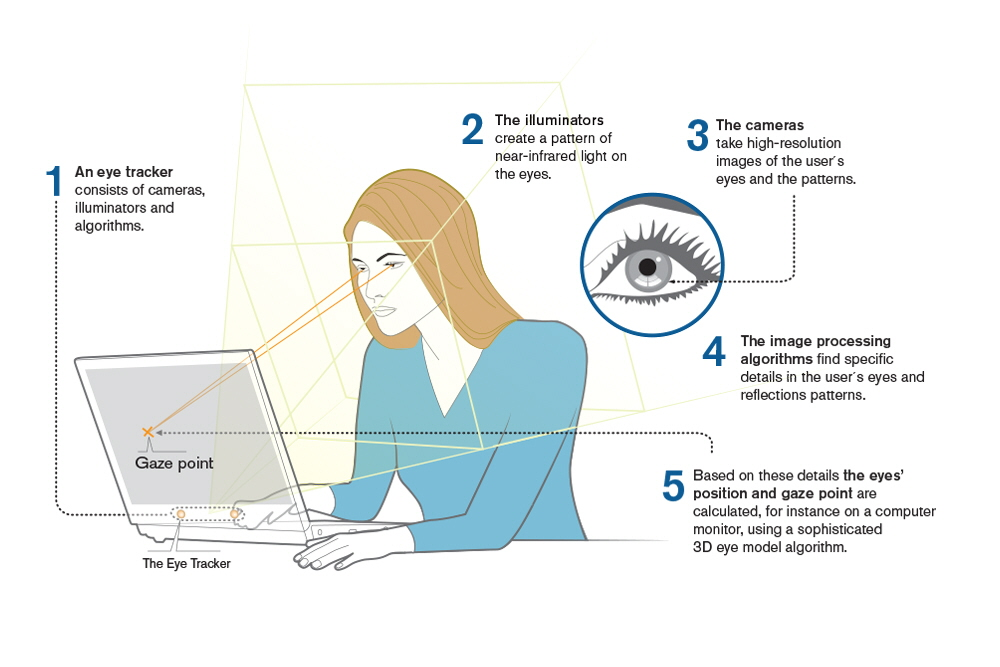
\includegraphics[width=1\textwidth]{../../Grafiken/How-20DoesEyetrackingWork_ScreenBased.jpg}
	\caption{Illustration der Funktionsweise von Tobii Pro Eyetracker. \cite{tobiipro}}
	\label{fig::et01}
\end{figure}
Dabei werden vier grundlegende Bestandteile des Eye Tracking, wie die Firma Tobii AB es realisiert, genannt.
In der Regel benötigt man für das Messen von Augenaktivitäten zwei grundlegende Dinge, die auch in Abbildung \ref{fig::et01} abgebildet sind: Eine Lichtquelle (2) und eine Kamera (3).
Es gibt verschiedene Möglichkeiten, die Augenaktivitäten zu messen.
Die am häufigsten genutzte Technik, welche auch von den Tobii Eyetrackern genutzt wird, ist \texttt{Pupil Centre Corneal Reflection (PCCR)}.
Die Lichtquellen sind dabei auf die Augen gerichtet und erzeugen auf ihnen ein spezielles Reflektionsmuster.
Die Kamera des Eyetrackers (3) nimmt mit einer hohen Abtastrate Bilder der Augen und ihrer Reflektionsmuster auf.
Nun können spezielle Bildverarbeitungsalgorithmen (4) auf die erfassten Daten angewendet werden und die Reflektionspunkte auf den Bildern bestimmt werden.
Anhand dieser Punkte und eines Modells des Auges kann die Blickrichtung der Augen, die Position der Augen im Raum und die Blickpunkte der Augen auf dem Bildschirm berechnet werden (4 + 5).
% \todo{Wie werden die Augen getrackt?}
% \todo{Wie sehen Messwerte aus und wie verwendet man sie richtig (Koordinatensysteme, Bildschirm und Fensteroffset.)}

\begin{figure}[]
	\centering
	\begin{minipage}[b]{0.49\textwidth}
		\centering
		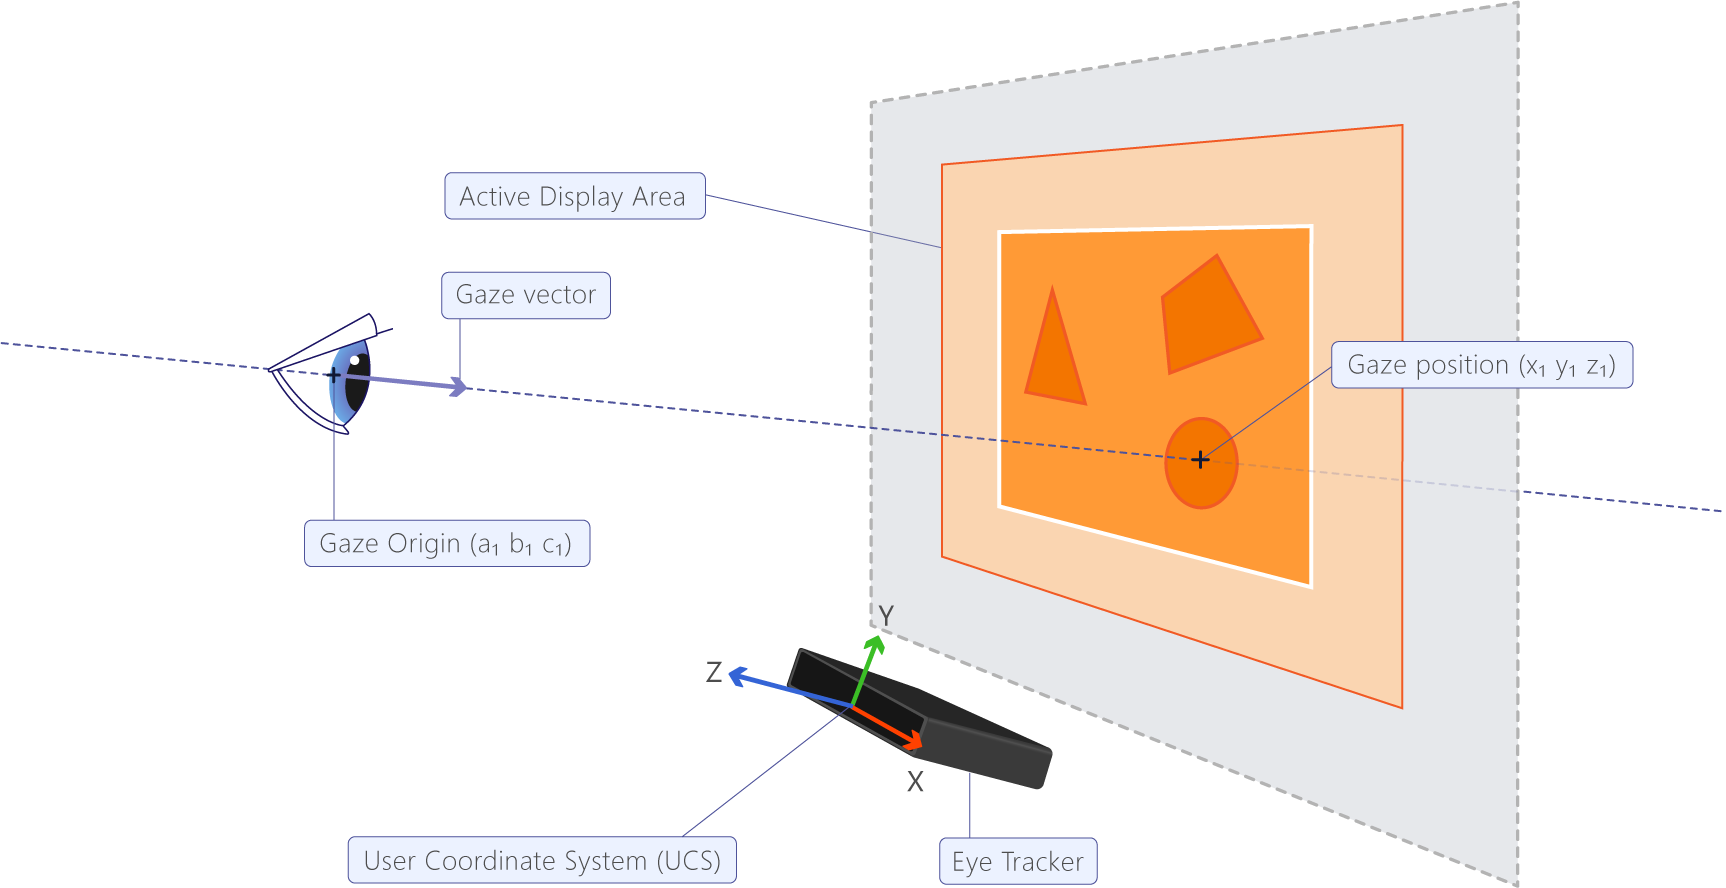
\includegraphics[width=1\textwidth]{../../Grafiken/UCS.png}
		\caption{Nutzer Koordinatensystem \cite{tobiisdk}}
		\label{fig::et02}
	\end{minipage}
	\hfill
	\begin{minipage}[b]{0.49\textwidth}
		\centering
		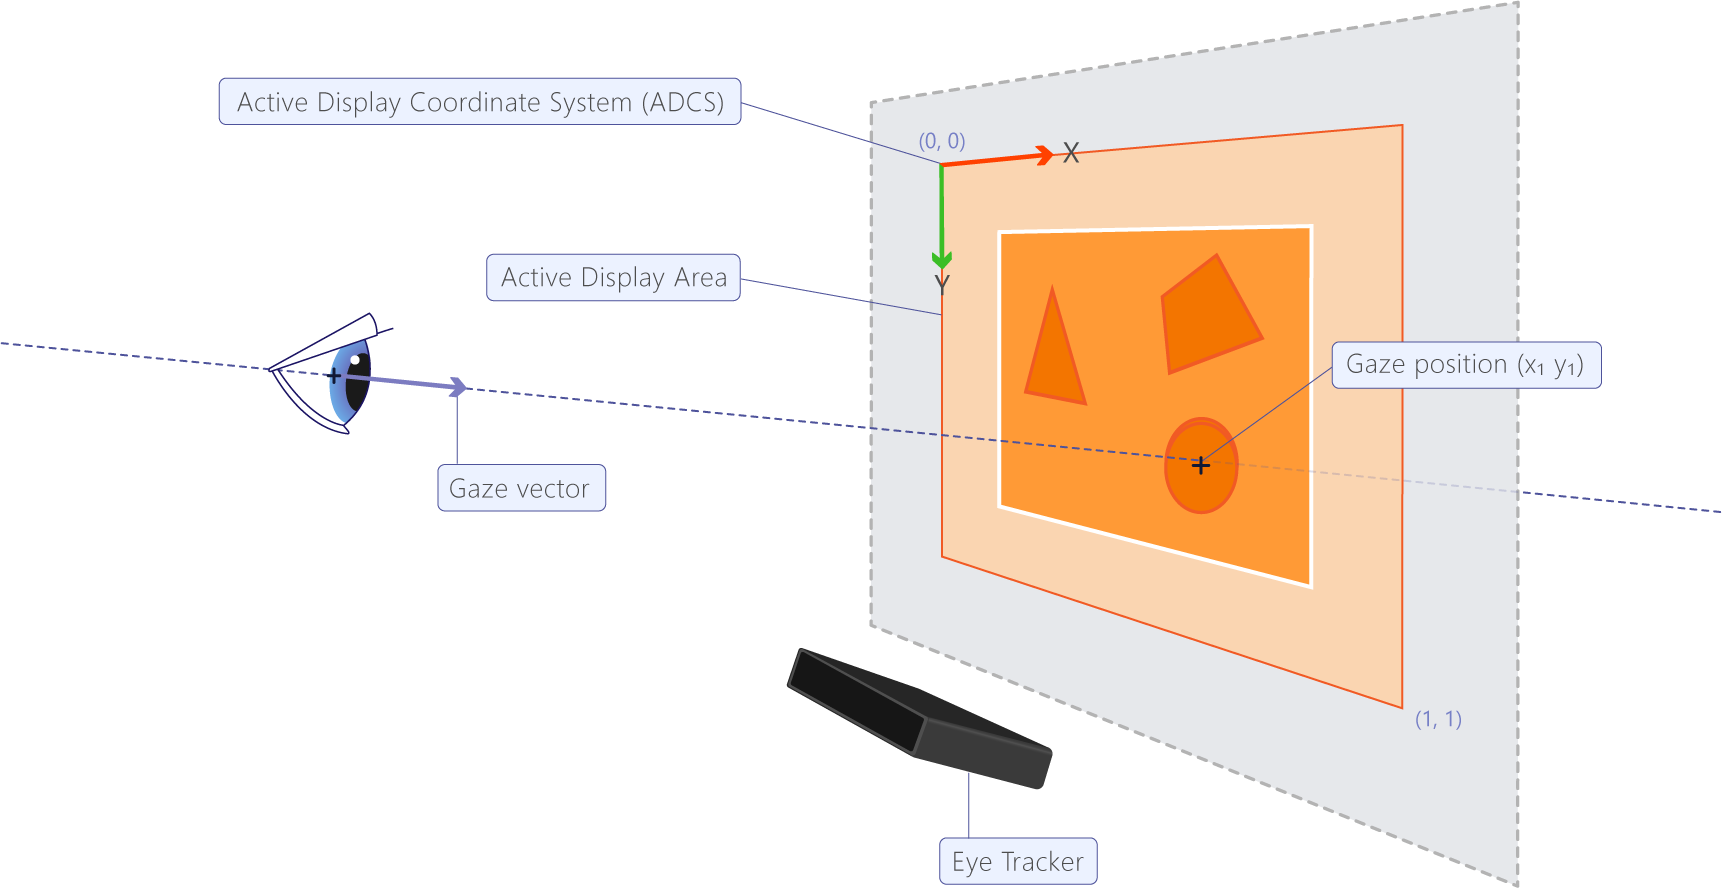
\includegraphics[width=1\textwidth]{../../Grafiken/ADCS.png}
		\caption{Aktives Display Koordinatensystem \cite{tobiisdk}}
		\label{fig::et03}
	\end{minipage}
\end{figure}
Die Position eines Auges im Raum wird als \texttt{Gaze origin} bezeichnet und wird bei Tobii Pro Eyetrackern im Nutzer Koordinatensystem angegeben, siehe Abbildung \ref{fig::et02}.
Der Blickpunkt des Auges auf dem Bildschirm ist in der Regel das, was von größtem Interesse ist und wird als \texttt{Gaze point} bezeichnet.
Der \texttt{Gaze point} wird im Aktiven Display Koordinatensystem angegeben, siehe Abbildung \ref{fig::et03}.
Dieses Koordinatensystem hat den Ursprung an der Position oben links des aktiven Bildschirmbereichs, und der Punkt (1,1) ist an der Position rechts unten des aktiven Bildschirmbereichs.
Die Umrechnung in Bildschirmkoordinaten funktioniert durch die Multiplikation mit der Breite und Höhe des Bildschirms in Pixel.
Die Koordinaten sind dann relativ zu dem aktiven Display.
Dieses Display muss nicht unbedingt das einzige Display sein.
Werden mehrere Bildschirme verwendet, muss möglicherweise ein Offset auf die Werte gerechnet werden, um die richtigen Bildschirmkoordinaten für den Bildschirm, auf dem die Anwendung dargestellt wird, zu erhalten.

%\todo{Umrechnung in Pixel und bei mehreren Bildschirmen.}
In Abschnitt \ref{sec::eye} wurden verschiedene Arten von Augenbewegungen angesprochen.
Eine sehr wichtige Rolle spielen dabei Fixationen und Sakkaden.
Bei der Analyse der visuellen Wahrnehmung des Menschen ergeben die Daten der Fixationen wichtige Informationen über Eigenschaften des visuellen Stimuli.
Bei einer Fixation fixieren die Augen einen gewissen Punkt für eine vergleichsweise lange Zeit (100ms - 1.5s) und können dadurch viele Informationen des fixierten Objekts erfassen.
Sakkaden hingegen sind kurze (20ms - 40ms) und schnelle Augenbewegungen zwischen zwei Fixationen.
Für wahrnehmungsorientierte interaktive Anwendungen ist es daher wichtig, eine hohe Abtastrate und niedrige Latenz bei der Erfassung der Augenaktivitäten zu haben.
Dies ermöglicht es, schnell zwischen einer Sakkade und Fixation zu unterscheiden und das nächste Bild, ohne eine merkbare Verzögerung und entsprechend des neuen Blickpunktes, darzustellen.
So sollte bei der Methode des wahrnehmungsorientierten Renderings, wobei nur in dem fovealen Bereich das Bild mit hoher Auflösung dargestellt wird, ein Update ca. zwischen 5ms bis 60ms nach der Augenbewegung gestartet worden sein, um eine Bildveränderung nicht zu bemerken.
Diese Zeit ist dabei abhängig davon, wie weit die unscharfe Fläche von der Fovea entfernt ist \cite{doi:10.1111/cgf.13150}.
%\begin{figure}
%	\centering
%	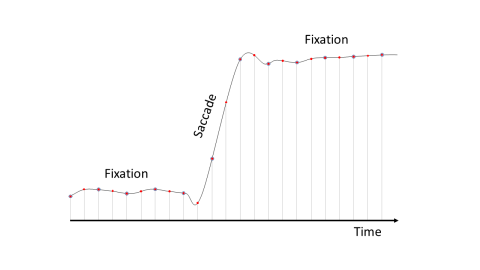
\includegraphics[width=0.5\textwidth]{../../Grafiken/Sampling-20frequency-201.png}
%	\caption{Abtastrate einer typischen Augenbewegung \cite{tobiisdk}}
%	\label{fig::et04}
%\end{figure}

Der in dieser Arbeit verwendete Tobii Pro Eyetracker hat eine Abtastfrequenz von 600 Hz.
Dies entspricht einem Abtastintervall von 1.67ms und ist vergleichsweise zu anderen aktuellen Eyetrackern recht hoch.
Diese haben oft eine Abtastfrequenz von 60 Hz oder 120 Hz.
Geräte mit Abtastraten im Frequenzbereich von 600 Hz und höher sind ausreichen schnell um Sakkaden messen zu können und haben eine entsprechend niedrige Latenz, welche es ermöglicht, eine Bildveränderung nicht wahrzunehmen.
\todo{Genaue Technische Daten des verwendeten Tobii Pro Eyetrackers nachschauen.}
Hohe Abtastraten heißt aber auch viele Daten pro Sekunde.
Für die Anwendung in dieser Arbeit ist es wichtig, den aktuellsten Blickpunkt des Auges zu kennen.
Daher wird der letzte gemessene gaze point des Eyetrackers für das Berechnen des nächsten Bildes verwendet.
Ein weiteres Problem bei vielen Messdaten ist es auch, dass es mehr fehlerhafte Messdaten gibt.
Die Daten, die über die Tobii Pro SDK durch den Eyetracker geliefert werden, enthalten dafür einen Validity Code.
Dieser Wert gibt an, ob eine Messung mit hoher Wahrscheinlichkeit richtige Daten enthält, oder nicht.
Dadurch können wahrscheinlich fehlerhafte Daten früh abgestoßen werden.
% \todo{Messgeschwindigkeit vs Augengeschwindigkeit}
% \todo{Validity Codes}
% \todo{Vorherige Todos ausschreiben und ggf. mehr.}

\section{GPU Architektur}\label{sec::gpuarc}
Ein wichtiger Faktor, wenn es um interaktive Anwendungen geht, ist die Performanz.
Viele Algorithmen haben essentielle Bestandteile welche ihre Komplexität nach unten beschränken.
Die Einführung von Parallelität ist ein wichtiger Ansatz, um die Performanz von Anwendungen beziehungsweise ihrer Algorithmen weiter zu verbessern.
Gerade Algorithmen in der Bildberechnung und -Verarbeitung eignen sich besonders um diese zu parallelisieren.
In der Bildverarbeitung werden viele gleiche Berechnungen auf unterschiedlichen Daten ausgeführt.
Graphics Processing Units (GPUs) oder auch Grafikkarten eignen sich für diese Art der Verwendung besonders.
\begin{figure}
	\centering
	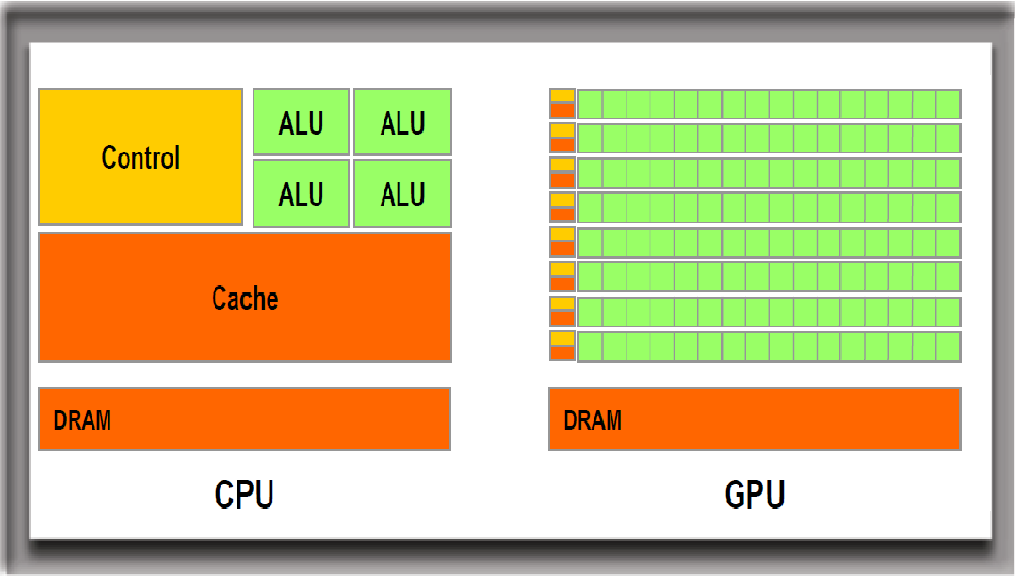
\includegraphics[width=0.5\textwidth]{../../Grafiken/CPU-GPU-Structures1.png}
	\caption{CPU vs. GPU. \url{http://www.keremcaliskan.com/wp-content/uploads/2011/01/CPU-GPU-Structures1.png}}
	\label{fig::ga01}
\end{figure}
% GPU vs CPU
Im Vergleich zu Central Processing Units (CPUs) besitzen GPUs eine deutlich höhere Anzahl an Prozessoren, siehe Abbildung \ref{fig::ga01}.
Aktuell besitzen Prozessoren meist vier oder acht Rechenkerne und eine Taktfrequenz von ca. 4 Ghz.
GPUs hingegen haben mehrere tausend Berechnungseinheiten die gleichzeitig Berechnungen durchführen können, dafür aber bei ca. einem drittel der Taktfrequenz von CPUs.

Fast jeder Computer besitzt heutzutage hochparallele Einheiten wie eine GPU.
In den Anfängen waren GPUs sehr eng mit grafischen Berechnungen verbunden um die Berechnung von Farbwerten von Pixeln zu beschleunigen.
Heute werden GPUs zur Beschleunigung von fast beliebigen Anwendungen genutzt.
Programmierschnittstellen wie OpenCL oder CUDA ermöglichen die Nutzung von GPUs für allgemeine Berechnungen, oder auch General Purpose Computation on Graphics Processing Unit (GPGPU).

\subsection*{OpenCL}
OpenCL (Open Computing Language) ist ein Standard für das allgemeine Programmieren für parallele CPU oder GPU-Platformen.
Dabei stellt OpenCL eine Programmierschnittstelle für das koordinieren paralleler Berechnungen auf unterschiedlichen Platformen zur Verfügung, sowie eine Programmiersprache für die eigentliche Programmierung von Programmen, die auf parallelen Platformen wie einer GPU ausgeführt werden sollen.

Eine OpenCL Anwendung ist die Kombination des Codes eines Programms, das auf dem Host und den OpenCL Devices ausgeführt wird.
Der Host ist dabei der Teil der Anwendung, der mit dem OpenCL Kontext über die OpenCL API kommuniziert.
Ein Kontext ist die Umgebung, in der ein OpenCL Kernel ausgeführt wird und weitere Eigenschaften definiert sind.
Der Kernel ist eine Funktion die in einem OpenCL Programm geschrieben wurde und durch ein OpenCL Device ausgeführt wird.
Ein Device entspricht meistens eine GPU oder CPU, die OpenCL implementiert. % bzw. deren Treiber OpenCL implementieren

\subsubsection*{OpenCL Platform Modell}
\begin{figure}
	\centering
	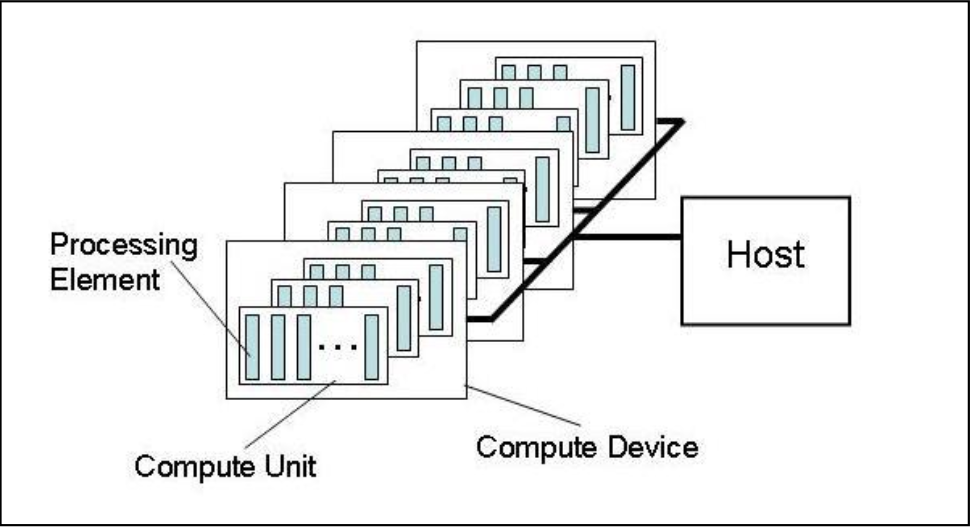
\includegraphics[width=0.5\textwidth]{../../Grafiken/OpenCL_PlatformModel.png}
	\caption{OpenCL Platform Modell ... ein Host, mehrere Compute Devices (ein Compute Device entspricht zum Beispiel einer GPU) mit je einer oder mehreren Compute Units. \url{https://www.khronos.org/registry/OpenCL/specs/opencl-2.1.pdf}}
	\label{fig::ga02}
\end{figure}
Das Platform Modell von OpenCL ist eine Abstraktion davon, wie OpenCL die Hardware sieht.
Die Beziehung zwischen seinen Einheiten und der Hardware ist dabei größtenteils von der verwendeten Hardware und ihrer Implementierung von OpenCL abhängig.
Es besteht aus einem Host, welcher mit ein oder mehreren Devices verbunden ist.
Diese sind unterteilt in Compute Units (CUs), welche weiter in Processing Elements (PEs) unterteilt sind.
Berechnungen auf einem solchen Device werden in Processing Elements ausgeführt.
Die Host-Anwendung gibt den Start des Kernel-Codes in Auftrag.
Das OpenCL Device führt dann den Kernel Code auf den Processing Elements des Devices aus und hat dabei eine große Freiheit darüber, wie die Berechnungen auf den Processing Elements abgebildet werden.
Falls die Processing Elements innerhalb einer Compute Unit die gleiche Folge von Befehlen ausführen, bezeichnet man ihren Befehlsfluss als konvergiert, sonst als divergiert.

\subsubsection*{OpenCL Ausführungsmodell}
Der Host kann über Funktionen der OpenCL API mit einem Device über eine Command-Queue interagieren.
Eine Command-Queue ist mit maximal einem Device verknüpft.
Über die Command-Queue können Befehle zum starten eines Kernels, Transferieren von Daten zwischen Host und Device und Befehle zur Synchronisation ausgeführt werden.
Ein Befehl durchläuft dabei immer sechs Zustände: Queued (Eingereiht), Submitted (Übermittelt), Ready (Bereit), Running (Ausführend), Ended (Beendet) und Complete (Abgeschlossen).
Wird ein Kernel für die Ausführung übermittelt, wird für diesen ein Index-Raum definiert.
Der Kernel selbst, die zugehörigen Parameter und die Parameter, die seinen Index-Raum definieren, definieren eine Kernel Instanz.
Wird eine Kernel Instanz auf dem Device ausgeführt, wird für jeden Punkt in seinem Index-Raum eine Ausführung des Kernels gestartet.
Eine solche Ausführung wird Work-Item genannt.
Work-Items, die zu einer bestimmten Kernel Instanz gehören, werden von dem Device in Gruppen gehandhabt.
Diese Gruppen heißen Work-Groups.

\begin{figure}
	\centering
	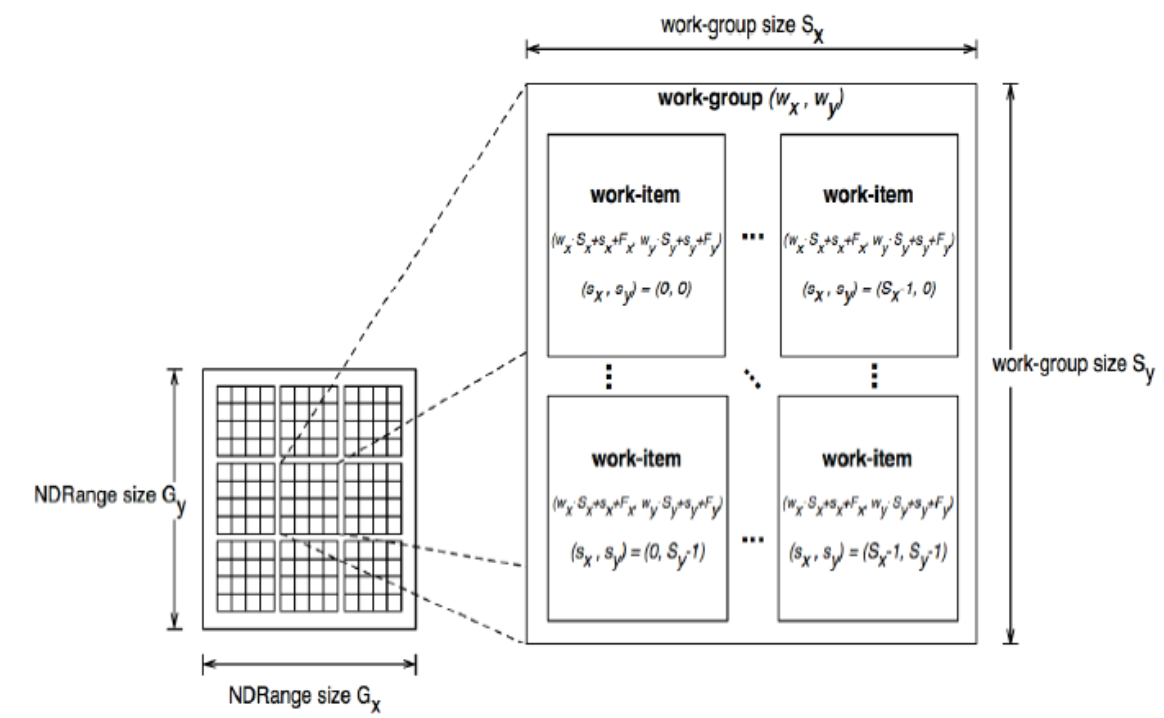
\includegraphics[width=0.75\textwidth]{../../Grafiken/OpenCL-NDRange-Mapping.png}
	\caption{OpenCL NDRange-Mapping. \url{https://www.khronos.org/registry/OpenCL/specs/opencl-2.1.pdf}}
	\label{fig::ga03}
\end{figure} 

\todo{Hardwarerealisierung, NVIDIA und AMD u.U. Intel}
\todo{Performanzoptimierung: Warp-Auslastung, Speicher-Blockierung}
